%%%%%%%%% NEW SECTION: INTRODUCTION %%%%%%%%%

\section{Introduction}
The CRIMI (Chris's Radio and Infrared Michelson Interferometer) is an infrared Fourier transform spectrometer, made by Chris de Jonge, under supervision of Dr. Andrey Baryshev. The spectrometer is designed to be used in a vacuum, as water molecules and other abundant molecules absorb large parts of the infrared spectrum.

The goal of this internship was to write software to guide the linear stage in the CRIMI in making measurements, design a graphical user interface for easy user access and do some data processing on the acquired data: fast Fourier transforms and windowing. As a result, I have written a program in Python that automatically takes a complete measurement with this spectrometer. The program has scan length and stepsize, or equivalent resolution and maximum frequency, for input, and outputs the raw data in \verb!csv! format.

%Doe hier ook een plaatje van een FTS (kun je van WIKIPEDIA halen). doel van je stage was:
%aansturing van linear stage
%grafische user interface
%data processing (FFT algorithmes + windowing)
%Zet in deze introductie ook een formule en plaatje met spectrum en interferogram.
\textbf{Verder is het goed om hier ook aan te geven hoe padlengte de resolutie bepaalt, en minimale stapgrootte de hoogste frequentie.}

\subsection{Fourier Transform}

Fourier transform spectrometers (FTS) work on the interference and Fourier principles. The spectrometer has a moveable part and stationary parts. In the case of figure~\ref{fig:fts}, a moving mirror provides a difference in distance travelled by the two beams of light created by the beamsplitter. By moving one mirror, the path length $l_1$ is made different from $l_2$, which produces an interference pattern when the light is recombined. Because of the range of wavelengths in the light, at different positions of the mirror, different wavelengths are attenuated.

With a Fourier transform the intensity for each position ($\delta$) is turned into the intensity for each wavenumber ($\tilde{\nu}$), because one is the inverse of the other: $\tilde{\nu} = \frac{1}{\delta}$, and from this the frequency $f$ can be computed: $\tilde{\nu}\cdot c=f$. $\delta$ and $\nu$ are together called a Fourier transform pair.

The Fourier transform of a function is the following formula:

\[
 F(\tilde{\nu})=\int_{-\infty}^{\infty}f(t)e^{-i\omega t}dt
\]
with $i$ the unit imaginary number.

\begin{figure}
 \begin{center}
  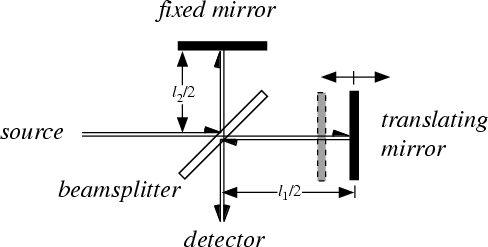
\includegraphics[width=0.8\textwidth]{figures/fts.png}
  \caption{A simple Fourier transform spectrometer (FTS). Path length differences are created by moving parts of the setup.  From \cite{wolf}.}
  \label{fig:fts}
 \end{center}
\end{figure}

\textbf{Zeg dingen over:}
\begin{itemize}
 \item Coherence of a light source
 \item To be more specific, between the light source and the detector, there is a certain configuration of mirrors that allows some wavelengths to pass through but blocks others (due to wave interference). The beam is modified for each new data point by moving one of the mirrors; this changes the set of wavelengths that can pass through.
As mentioned, computer processing is required to turn the raw data (light intensity for each mirror position) into the desired result (light intensity for each wavelength). The processing required turns out to be a common algorithm called the Fourier transform (hence the name, "Fourier transform spectroscopy"). The raw data is sometimes called an "interferogram". \textbf{Copypasta van wikipedia, AANPASSEN}
 \item Fourier transform $\rightarrow$ padlengte bepaalt resolutie, minimale stapgrootte de hoogste frequentie

\end{itemize}



\begin{figure}
 \begin{center}
  \subfloat[The measured interferogram.]{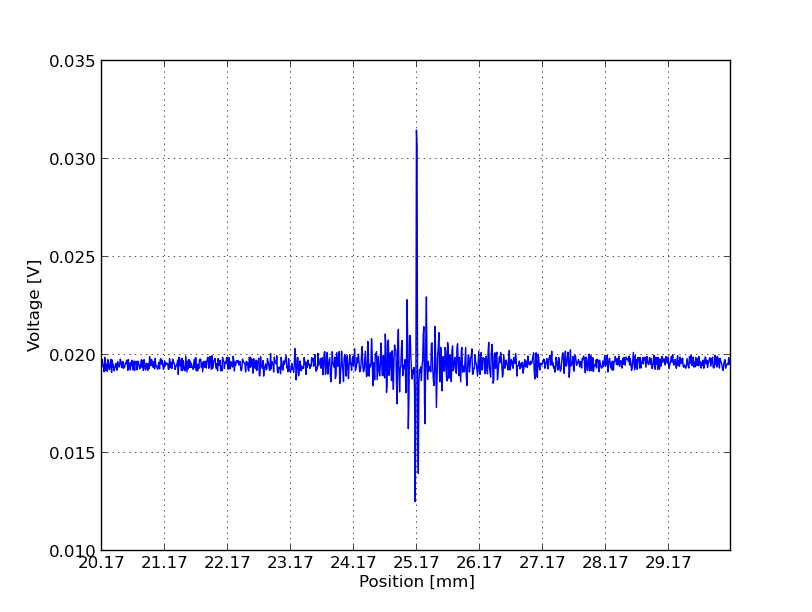
\includegraphics[width = 0.47\textwidth]{figures/interferogramforreport.png}}
  \quad
  \subfloat[The spectrum.]{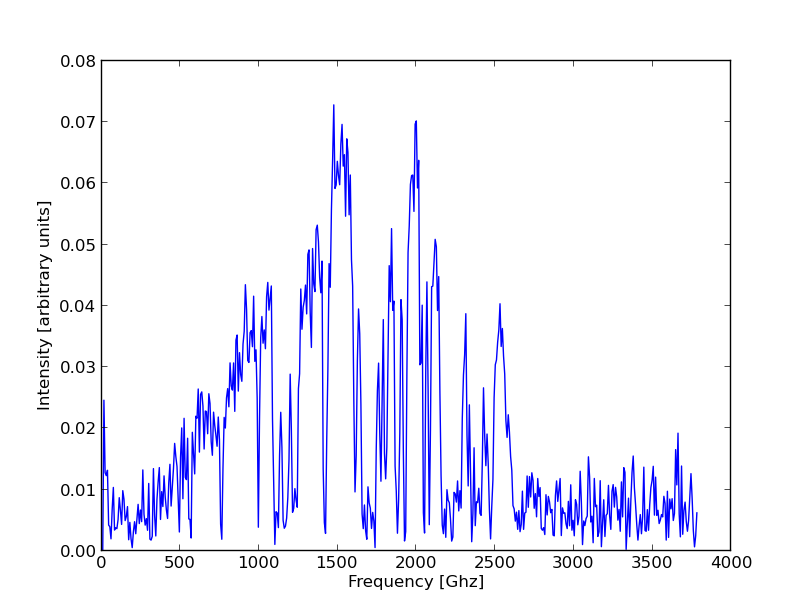
\includegraphics[width = 0.47\textwidth]{figures/fourierplotforreport.png}}
  \caption{The Fourier transform of an interferogram gives the spectrum.}
  \label{fig:fouriertransform}
 \end{center}
\end{figure}

\begin{itemize}
%\item Algemene inleiding over de CRIMI. (sortof done)
\item Iets met dat het programma voor windows geschreven is (serial ports zijn com-ports).
%z\item dingen over waarom een fts gebruiken (fourier $\rightarrow$ dus informatie over meerdere frequenties in 1x).
%\item \textbf{check measurement 20121005-1725!}
%\item something about the lock in technique? Nope, niet relevant voor programma.
\end{itemize}

\subsection{Hardware}

The spectrometer needs a few devices to function (see figure \ref{fig:hardware}). The controller to move the stage in is the PI C867.160 controller. The lock in amplifier in use is the SR510. A third device is needed to be able to communicate with the lock in amplifier from any computer: a GPIB-Ethernet adapter. This device counteracts the need for a special GPIB circuit card in the computer. All three are hardcoded into the software. This means unfortunately that the software does not automatically work with e.g. the SR530 lock in amplifier, or with a direct GPIB connection to the computer.

The test setup used a helium-cooled bolometer to actually measure the power of the radiation. This report will not deal any further with the measuring device, as the software is independent of that.


\begin{figure}[h!tb]
	\begin{center}
		\subfloat[The controller for the stage from PI.]{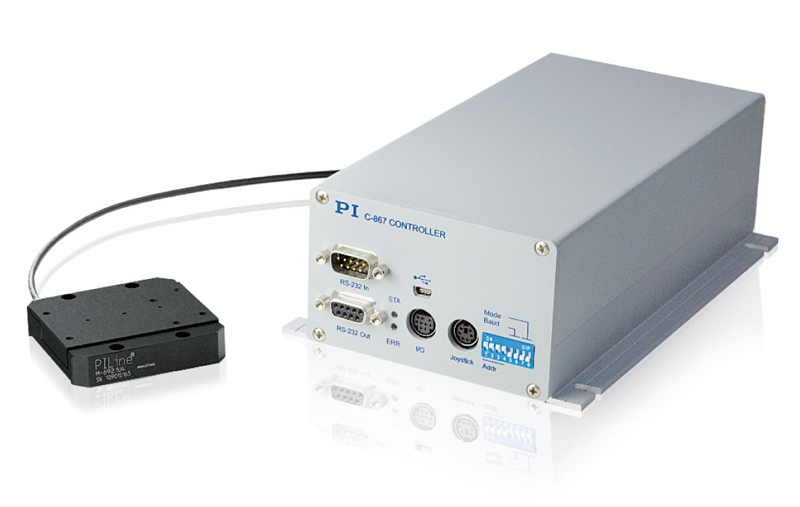
\includegraphics[width = 0.45\textwidth]{figures/pi_c867_160.jpg}}
		\qquad
		\subfloat[The SR510 lock in amplifier.]{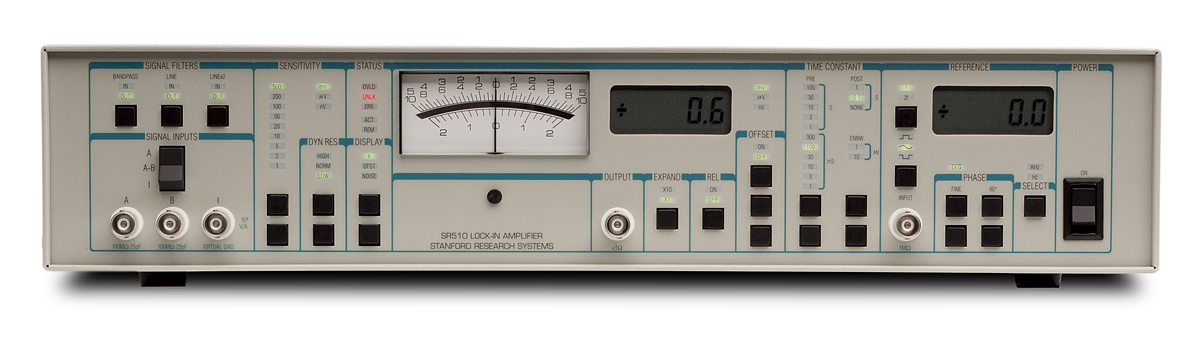
\includegraphics[width = 0.45\textwidth]{figures/SR510_FPlg.jpg}}
		\qquad
		\subfloat[The GPIB-Ethernet Controller.]{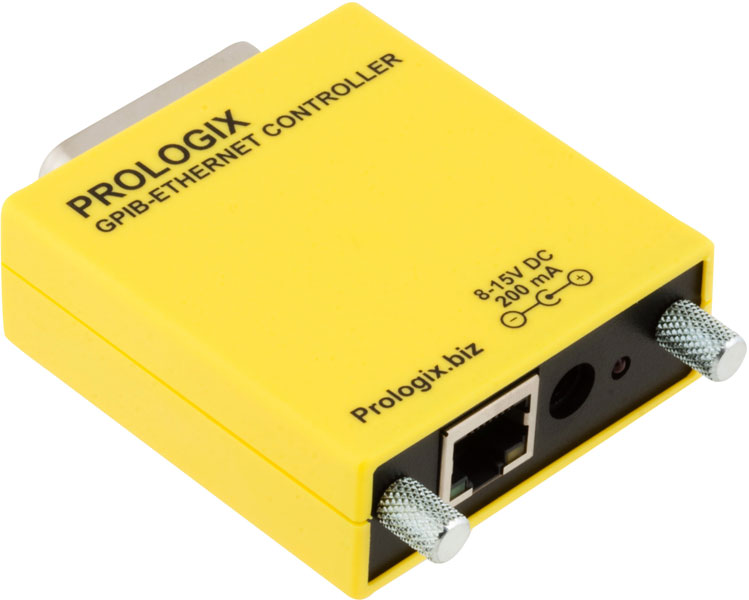
\includegraphics[width = 0.4\textwidth]{figures/GPIB-Ethernet-back.jpg}}
		\caption{The hardware. Pictures from \cite{PI}, \cite{SR}, and \cite{prologix}.}
		\label{fig:hardware}
	\end{center}
\end{figure}

It is important to mention that on the SR510 the DIP-switches need to be in a different configuration than the `example' configuration as mentioned in its manual on page 7. For fast readout, SW1 switch 6 should be in the `up' position instead of in the `down' position, to suppress echoing over the RS232 connection (which is unconnected in this setup). The SW2 switches are not of importance in this setup, as no RS232 connection is used. See figure~\ref{fig:SR510_back} for the location of this switch.

\begin{figure}
 \begin{center}
  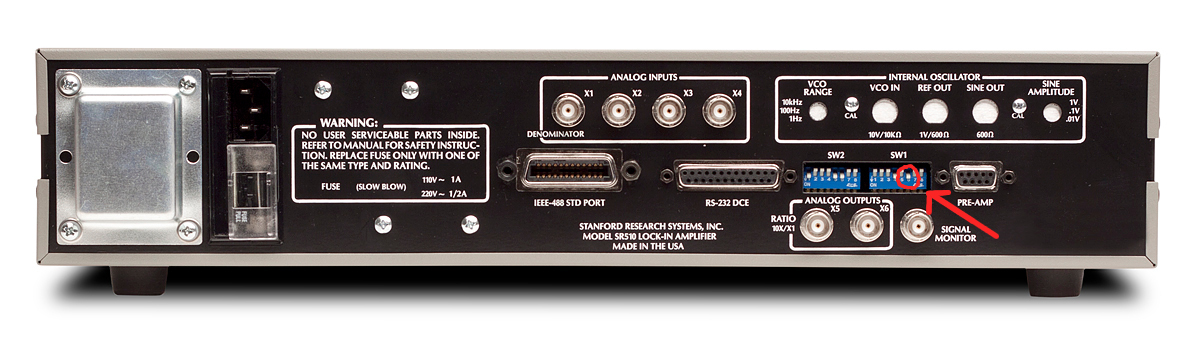
\includegraphics[width=\textwidth]{figures/SR510_Rear_circle.jpg}
  \caption{The back plate of the SR510 lock in amplifier. Encircled is SW1 switch 6. For fast performance, this switch should be in the `up' position. Picture from \cite{SR}.}
  \label{fig:SR510_back}
 \end{center}
\end{figure}


\subsection{Python}
Python is an interpreted, interactive, object-oriented programming language \cite{python}. It is open source and free, and easy to learn. Python runs on Windows, Linux/Unix and Mac OS X. It has an active community that contributes a large number of libraries for various tasks, e.g. numerical mathematics and hardware interfacing.

Python has the distinct advantage over programming languages such as LabVIEW that it is backwards compatible. Old code written in previous versions is in many cases still executable in newer Python versions, and as the files are plain text, it will be always readable in any editor. So even when old code cannot be executed anymore, it can still be modified to comply with newer standards.

This software is written in Python version 2.7. The extra (non-native) packages needed for the program are \verb!PySerial! to open a serial port for the PI-controller and \verb!wxPython! to make the GUI. For this last task \verb!wxFormbuilder!, an open source GUI designer which emits Python code, was also used. The other imported packages are part of the core Python distribution.
